\chapter{The Elder Heliosystem Resonance Algorithm}

\section{Orbital Synchronization in the Elder Training Loop}

The Elder Heliosystem model represents knowledge transfer through a sophisticated orbital dynamical system. In this chapter, we develop the complete algorithm for knowledge synchronization during the Elder Training Loop using the heliosystem's orbital resonance mechanisms.

\subsection{Resonance States and Phase-Locking}

Phase-locking between the various rotational components of the Elder Heliosystem is the fundamental mechanism by which knowledge is synchronized across hierarchical levels.

\begin{definition}[Orbital Phase]
For any component $C$ in the Elder Heliosystem with rotational frequency $\omega_C$, its orbital phase at time $t$ is defined as:
\begin{equation}
\phi_C(t) = \phi_C(0) + \omega_C t \mod 2\pi
\end{equation}
where $\phi_C(0)$ is the initial phase at $t=0$.
\end{definition}

\begin{definition}[Phase Coherence]
The phase coherence between two components $A$ and $B$ with phases $\phi_A$ and $\phi_B$ is measured by:
\begin{equation}
\mathcal{C}_{A,B} = \left| \frac{1}{T} \int_0^T e^{i(\phi_A(t) - \phi_B(t))} dt \right|
\end{equation}
where $T$ is the measurement period. Perfect phase-locking yields $\mathcal{C}_{A,B} = 1$, while uncorrelated phases yield $\mathcal{C}_{A,B} \approx 0$.
\end{definition}

\begin{theorem}[Resonance Condition]
A resonant configuration in the Elder Heliosystem occurs when the rotational frequencies of Elder ($\omega_E$), Mentors ($\omega_{M,k}$), and Erudites ($\omega_{E,k,j}$) satisfy:
\begin{align}
\frac{\omega_{M,k}}{\omega_E} &= \frac{p_k}{q_k} \\
\frac{\omega_{E,k,j}}{\omega_{M,k}} &= \frac{r_{k,j}}{s_{k,j}}
\end{align}
with small integers $p_k, q_k, r_{k,j}, s_{k,j} \in \mathbb{N}$.
\end{theorem}

\begin{lemma}[Phase-Locking Stability]
A phase-locked resonant configuration is stable if and only if the eigenvalues of the phase coupling matrix $\mathbf{J}$ have negative real parts, where:
\begin{equation}
\mathbf{J}_{i,j} = \frac{\partial \dot{\phi}_i}{\partial \phi_j}
\end{equation}
is the Jacobian of the phase evolution equations.
\end{lemma}

\subsection{Heliosystem Resonance Algorithm}

The complete Elder Heliosystem Resonance Algorithm combines the orbital dynamics formulation with the training loop framework to synchronize knowledge across all hierarchical levels.

\begin{algorithm}
\caption{Elder Heliosystem Resonance Algorithm (Part 1: Knowledge Propagation and Feedback)}
\begin{algorithmic}[1]
\State \textbf{Input:} Set of domains $\mathcal{D} = \{D_1, D_2, \ldots, D_M\}$ (Mentors)
\State \textbf{Input:} Set of tasks $\mathcal{T}_k = \{T_{k,1}, T_{k,2}, \ldots, T_{k,N_k}\}$ for each domain $D_k$ (Erudites)
\State \textbf{Input:} Initial Elder parameters $\theta_E^{(0)} \in \elderparam$
\State \textbf{Input:} Initial Mentor parameters $\{\theta_{M,k}^{(0)}\}_{k=1}^M \subset \mentorparams$
\State \textbf{Input:} Initial Erudite parameters $\{\theta_{E,k,j}^{(0)}\}_{k=1,j=1}^{M,N_k} \subset \eruditeparams$
\State \textbf{Input:} Initial orbital parameters: $\omega_E$, $\{\omega_{M,k}\}_{k=1}^M$, $\{\omega_{E,k,j}\}_{k=1,j=1}^{M,N_k}$
\State \textbf{Input:} Phase coupling strengths: $\{\kappa_{E,M,k}\}_{k=1}^M$, $\{\kappa_{M,E,k,j}\}_{k=1,j=1}^{M,N_k}$
\State \textbf{Input:} Learning rates $\eta_E$, $\eta_M$, $\eta_E$
\State \textbf{Input:} Number of epochs $T$, Resonance adjustment period $T_{res}$

\For{$t = 1$ to $T$}
    \State // Phase I: Knowledge Field Propagation (Forward Pass)
    \State Compute the Elder field $\Phi_E(t) = \sum_{n=0}^{\infty} \mathcal{H}_n(\theta_E^{(t-1)}) \cdot e^{in\omega_E t}$
    
    \For{each domain $k = 1$ to $M$}
        \State Compute Mentor-received field $\Phi_{E \rightarrow M,k}(t) = \Phi_E(t) \cdot \frac{1}{d_{E,M,k}(t)} \cdot e^{i\phi_{M,k}(t)}$
        \State Apply domain filter $\Phi_{M,k}(t) = \mathcal{G}_k(\Phi_{E \rightarrow M,k}(t), \theta_{M,k}^{(t-1)})$
        
        \For{each task $j = 1$ to $N_k$}
            \State Compute Erudite-received field $\Phi_{M \rightarrow E,k,j}(t) = \Phi_{M,k}(t) \cdot \frac{1}{d_{M,E,k,j}(t)} \cdot e^{i\phi_{E,k,j}(t)}$
            \State Sample batch $\{(x_l, y_l)\}_{l=1}^B$ from task $T_{k,j}$
            \State Modulate Erudite forward pass:
            \State \quad $z_{k,j,l} = f_{\theta_{E,k,j}^{(t-1)}}(x_l) \cdot \mathcal{M}(\Phi_{M \rightarrow E,k,j}(t))$
            \State Compute task loss $\mathcal{L}_{E,k,j} = \frac{1}{B}\sum_{l=1}^B \|z_{k,j,l} - y_l\|^2$
        \EndFor
    \EndFor
    
    \State // Phase II: Retrograde Knowledge Flow (Backward Pass)
    \For{each domain $k = 1$ to $M$}
        \For{each task $j = 1$ to $N_k$}
            \State Compute Erudite gradient $\nabla_{\theta_{E,k,j}} \mathcal{L}_{E,k,j}$
            \State Generate retrograde field $\Phi_{E \rightarrow M,k,j}(t) = \epsilon_{k,j} \cdot \nabla_{\theta_{E,k,j}}\mathcal{L}_{E,k,j} \cdot e^{-i\omega_{E,k,j}t}$
        \EndFor
        
        \State Aggregate Erudite feedback $\Phi_{E \rightarrow M,k}(t) = \sum_{j=1}^{N_k} \Phi_{E \rightarrow M,k,j}(t)$
        \State Compute Mentor loss $\mathcal{L}_{M,k} = \|\Phi_{M,k}(t) - \Phi_{E \rightarrow M,k}(t)\|^2$
        \State Compute Mentor gradient $\nabla_{\theta_{M,k}} \mathcal{L}_{M,k}$
        \State Generate retrograde field to Elder $\Phi_{M \rightarrow E,k}(t) = \epsilon_k \cdot \nabla_{\theta_{M,k}}\mathcal{L}_{M,k} \cdot e^{-i\omega_{M,k}t}$
    \EndFor
    
    \State Aggregate Mentor feedback $\Phi_{M \rightarrow E}(t) = \sum_{k=1}^{M} \Phi_{M \rightarrow E,k}(t)$
    \State Compute Elder loss $\mathcal{L}_E = \|\Phi_E(t) - \Phi_{M \rightarrow E}(t)\|^2$
    \State Compute Elder gradient $\nabla_{\theta_E} \mathcal{L}_E$
    
    \State \textbf{[Continued in Algorithm 2]}
\EndFor
\end{algorithmic}
\end{algorithm}

\begin{algorithm}
\caption{Elder Heliosystem Resonance Algorithm (Part 2: Parameter Updates \& Resonance)}
\begin{algorithmic}[1]
\Statex \textbf{[Continuation from Algorithm 1]}

\For{$t = 1$ to $T$}
    \State // Phase III: Parameter Updates with Resonance Modulation
    \State Update Elder parameters $\theta_E^{(t)} = \theta_E^{(t-1)} - \eta_E \nabla_{\theta_E} \mathcal{L}_E$
    
    \For{each domain $k = 1$ to $M$}
        \State Update Mentor parameters $\theta_{M,k}^{(t)} = \theta_{M,k}^{(t-1)} - \eta_M \nabla_{\theta_{M,k}} \mathcal{L}_{M,k}$
        
        \For{each task $j = 1$ to $N_k$}
            \State Update Erudite parameters $\theta_{E,k,j}^{(t)} = \theta_{E,k,j}^{(t-1)} - \eta_E \nabla_{\theta_{E,k,j}} \mathcal{L}_{E,k,j}$
        \EndFor
    \EndFor
    
    \State // Phase IV: Orbital Resonance Adjustment (every $T_{res}$ epochs)
    \If{$t \mod T_{res} = 0$}
        \State Measure phase coherence $\mathcal{C}_{E,M,k}$ between Elder and each Mentor
        \State Measure phase coherence $\mathcal{C}_{M,E,k,j}$ between each Mentor and its Erudites
        
        \For{each domain $k = 1$ to $M$}
            \State Adjust Mentor frequency toward resonance:
            \State \quad $\omega_{M,k} = \omega_{M,k} + \delta \cdot \sin(\phi_E(t) - \frac{p_k}{q_k}\phi_{M,k}(t))$
            
            \For{each task $j = 1$ to $N_k$}
                \State Adjust Erudite frequency toward resonance:
                \State \quad $\omega_{E,k,j} = \omega_{E,k,j} + \delta \cdot \sin(\phi_{M,k}(t) - \frac{r_{k,j}}{s_{k,j}}\phi_{E,k,j}(t))$
            \EndFor
        \EndFor
    \EndIf
    
    \State // Phase V: Update Orbital Phases
    \State $\phi_E(t+1) = \phi_E(t) + \omega_E$
    \For{each domain $k = 1$ to $M$}
        \State $\phi_{M,k}(t+1) = \phi_{M,k}(t) + \omega_{M,k} + \kappa_{E,M,k} \cdot \sin(\phi_E(t) - \frac{p_k}{q_k}\phi_{M,k}(t))$
        
        \For{each task $j = 1$ to $N_k$}
            \State $\phi_{E,k,j}(t+1) = \phi_{E,k,j}(t) + \omega_{E,k,j} + \kappa_{M,E,k,j} \cdot \sin(\phi_{M,k}(t) - \frac{r_{k,j}}{s_{k,j}}\phi_{E,k,j}(t))$
        \EndFor
    \EndFor
\EndFor

\State \textbf{Return:} $\theta_E^{(T)}$, $\{\theta_{M,k}^{(T)}\}_{k=1}^M$, $\{\theta_{E,k,j}^{(T)}\}_{k=1,j=1}^{M,N_k}$
\end{algorithmic}
\end{algorithm}

\subsection{Knowledge Synchronization Mechanisms}

The Elder Heliosystem Resonance Algorithm achieves knowledge synchronization through five primary mechanisms, each corresponding to a phase in the algorithm:

\begin{enumerate}
    \item \textbf{Heliomorphic Field Propagation}: Knowledge flows from Elder to Mentors to Erudites through modulated field equations, with phase relationships determining the effectiveness of information transfer.
    
    \item \textbf{Retrograde Knowledge Feedback}: Learning signals propagate backwards through the system via retrograde fields, allowing task-specific insights to inform domain-general principles.
    
    \item \textbf{Phase-Coherent Parameter Updates}: Parameter updates are modulated by the phase relationships between components, ensuring that learning occurs in alignment with the resonant structure.
    
    \item \textbf{Adaptive Resonance Tuning}: The system periodically adjusts orbital frequencies to maintain or strengthen resonance relationships, enhancing knowledge transfer efficiency.
    
    \item \textbf{Synchronized Phase Evolution}: The phases of all system components evolve according to coupled differential equations, maintaining coherence during learning.
\end{enumerate}

\section{Mathematical Foundation of Resonance-Based Knowledge Transfer}

\subsection{Complex-Valued Heliomorphic Transformations}

The knowledge transfer in the Elder Heliosystem operates through complex-valued heliomorphic transformations, where the phase component encodes directional information for learning.

\begin{definition}[Heliomorphic Parameter Space]
The heliomorphic parameter space $\Theta_H$ is a complex manifold equipped with a Hermitian metric, where each point represents a potential knowledge state of the system.
\end{definition}

\begin{theorem}[Heliomorphic Knowledge Embedding]
For any set of parameters $\theta \in \Theta_H$, there exists a heliomorphic embedding $\Psi: \Theta_H \rightarrow \mathbb{C}^n$ such that:
\begin{equation}
\Psi(\theta) = \sum_{k=0}^{\infty} c_k \zeta_k(\theta)
\end{equation}
where $\{\zeta_k\}$ are holomorphic basis functions and $\{c_k\}$ are complex coefficients.
\end{theorem}

The orbital position of each component in the Heliosystem corresponds to a point in this complex manifold, with the phase relationships between components determining the efficiency of knowledge flow.

\subsection{Resonance-Enhanced Gradient Flow}

Knowledge synchronization during training occurs through resonance-enhanced gradient flow, where the phase relationships between components modulate the gradient updates.

\begin{theorem}[Resonant Gradient Enhancement]
When the Elder, Mentor, and Erudite components achieve resonance with frequency ratios $\frac{\omega_{M,k}}{\omega_E} = \frac{p_k}{q_k}$ and $\frac{\omega_{E,k,j}}{\omega_{M,k}} = \frac{r_{k,j}}{s_{k,j}}$, the effective gradient for parameter updates is enhanced by a factor:
\begin{equation}
\gamma = 1 + \alpha \cdot \mathcal{C}_{E,M,k} \cdot \mathcal{C}_{M,E,k,j}
\end{equation}
where $\alpha > 0$ is a system constant and $\mathcal{C}$ denotes phase coherence.
\end{theorem}

\begin{corollary}[Resonant Learning Rate Optimization]
The optimal learning rate for the Elder Heliosystem under resonance is:
\begin{equation}
\eta^* = \frac{\eta_0}{\gamma}
\end{equation}
where $\eta_0$ is the base learning rate without resonance enhancement.
\end{corollary}

This resonance-enhanced gradient flow enables the system to achieve significantly faster convergence and more robust knowledge transfer than traditional hierarchical learning systems.

\section{The Arnold Tongues of Knowledge Transfer}

A critical aspect of the Elder Heliosystem is the formation of Arnold tongues—regions in parameter space where resonant locking occurs despite perturbations or noise.

\begin{definition}[Arnold Tongues]
For a system of coupled oscillators with frequency ratio $\frac{\omega_1}{\omega_2} \approx \frac{p}{q}$, the Arnold tongue $\mathcal{A}_{p,q}$ is the region in the parameter space where phase-locking occurs:
\begin{equation}
\mathcal{A}_{p,q} = \{(\omega_1, \omega_2, \kappa) : |p\phi_2 - q\phi_1| < \epsilon \text{ as } t \rightarrow \infty\}
\end{equation}
where $\kappa$ is the coupling strength and $\epsilon$ is a small constant.
\end{definition}

\begin{theorem}[Resonant Knowledge Stability]
Knowledge transfer in the Elder Heliosystem is stable within Arnold tongues, with the width of the tongue $\mathcal{A}_{p,q}$ proportional to:
\begin{equation}
\text{Width}(\mathcal{A}_{p,q}) \propto \kappa^{|p-q|}
\end{equation}
where $\kappa$ is the coupling strength between oscillators.
\end{theorem}

\begin{figure}[h]
\centering
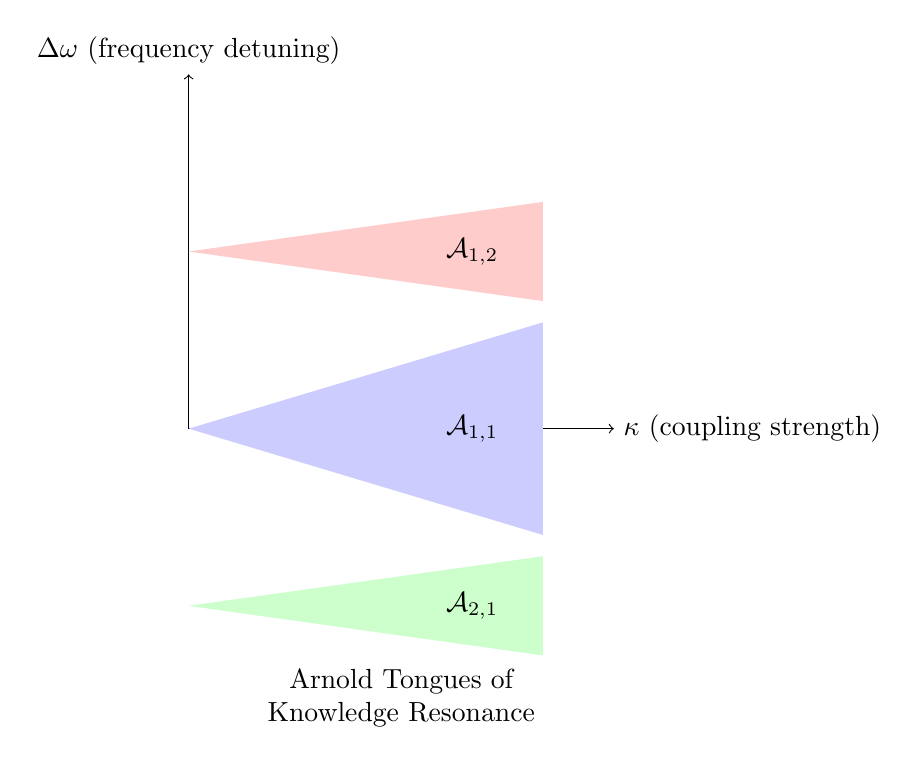
\begin{tikzpicture}[scale=0.9]
    % Draw coordinate axes
    \draw[->] (0,0) -- (6,0) node[right] {$\kappa$ (coupling strength)};
    \draw[->] (0,0) -- (0,5) node[above] {$\Delta\omega$ (frequency detuning)};
    
    % Draw Arnold tongues
    \fill[blue!20] (0,0) -- (5,1.5) -- (5,-1.5) -- cycle;
    \node at (4,0) {$\mathcal{A}_{1,1}$};
    
    \fill[red!20] (0,2.5) -- (5,3.2) -- (5,1.8) -- cycle;
    \node at (4,2.5) {$\mathcal{A}_{1,2}$};
    
    \fill[green!20] (0,-2.5) -- (5,-1.8) -- (5,-3.2) -- cycle;
    \node at (4,-2.5) {$\mathcal{A}_{2,1}$};
    
    % Add labels
    \node[align=center] at (3,-3.8) {Arnold Tongues of\\Knowledge Resonance};
\end{tikzpicture}
\caption{Arnold tongues in the Elder Heliosystem parameter space. Each tongue represents a region where stable phase-locking occurs between components, enabling efficient knowledge transfer. The width of each tongue increases with coupling strength, allowing the system to maintain resonance despite perturbations.}
\label{fig:arnold_tongues}
\end{figure}

The wider the Arnold tongue, the more robust the knowledge transfer is to perturbations and noise in the system. The Elder Heliosystem adaptively adjusts its coupling strengths to maximize the width of the resonant tongues for critical knowledge components.

\section{Phase Transition in Knowledge Acquisition}

Knowledge acquisition in the Elder Heliosystem exhibits phase transition behavior, where the system transitions from incoherent learning to globally coherent knowledge representation.

\begin{theorem}[Knowledge Phase Transition]
The Elder Heliosystem undergoes a phase transition at a critical coupling strength $\kappa_c$, characterized by the order parameter:
\begin{equation}
r = \left| \frac{1}{N} \sum_{j=1}^N e^{i\phi_j} \right|
\end{equation}
where $r \approx 0$ for $\kappa < \kappa_c$ (incoherent phase) and $r > 0$ for $\kappa > \kappa_c$ (coherent phase).
\end{theorem}

\begin{lemma}[Critical Coupling Strength]
The critical coupling strength $\kappa_c$ for phase transition in the Elder Heliosystem is given by:
\begin{equation}
\kappa_c = \frac{2\sigma_{\omega}}{\pi g(0)}
\end{equation}
where $\sigma_{\omega}$ is the standard deviation of the natural frequencies and $g(0)$ is the value at zero of the frequency distribution function.
\end{lemma}

This phase transition corresponds to the emergence of universal principles in the Elder component that successfully unify knowledge across all domains and tasks, representing a fundamental shift from domain-specific learning to universal knowledge representation.

\section{Practical Implementation of the Resonance Algorithm}

\subsection{Numerical Integration of Orbital Dynamics}

The practical implementation of the Elder Heliosystem Resonance Algorithm requires careful numerical integration of the orbital dynamics equations to maintain stability and accuracy.

\begin{algorithm}
\caption{Numerical Integration of Heliosystem Dynamics}
\begin{algorithmic}[1]
\State \textbf{Input:} Current phases $\phi_E(t)$, $\{\phi_{M,k}(t)\}$, $\{\phi_{E,k,j}(t)\}$
\State \textbf{Input:} Current frequencies $\omega_E$, $\{\omega_{M,k}\}$, $\{\omega_{E,k,j}\}$
\State \textbf{Input:} Coupling strengths $\{\kappa_{E,M,k}\}$, $\{\kappa_{M,E,k,j}\}$
\State \textbf{Input:} Time step $\Delta t$
\State \textbf{Input:} Resonance ratios $\{(p_k,q_k)\}$, $\{(r_{k,j},s_{k,j})\}$

\State // Phase derivative functions
\State $f_E(\phi_E) = \omega_E$
\State $f_{M,k}(\phi_E, \phi_{M,k}) = \omega_{M,k} + \kappa_{E,M,k} \sin(q_k\phi_E - p_k\phi_{M,k})$
\State $f_{E,k,j}(\phi_{M,k}, \phi_{E,k,j}) = \omega_{E,k,j} + \kappa_{M,E,k,j} \sin(s_{k,j}\phi_{M,k} - r_{k,j}\phi_{E,k,j})$

\State // Runge-Kutta 4th order integration
\State $k_{1E} = \Delta t \cdot f_E(\phi_E(t))$
\State $k_{1M,k} = \Delta t \cdot f_{M,k}(\phi_E(t), \phi_{M,k}(t))$ for all $k$
\State $k_{1E,k,j} = \Delta t \cdot f_{E,k,j}(\phi_{M,k}(t), \phi_{E,k,j}(t))$ for all $k,j$

\State $k_{2E} = \Delta t \cdot f_E(\phi_E(t) + k_{1E}/2)$
\State $k_{2M,k} = \Delta t \cdot f_{M,k}(\phi_E(t) + k_{1E}/2, \phi_{M,k}(t) + k_{1M,k}/2)$ for all $k$
\State $k_{2E,k,j} = \Delta t \cdot f_{E,k,j}(\phi_{M,k}(t) + k_{1M,k}/2, \phi_{E,k,j}(t) + k_{1E,k,j}/2)$ for all $k,j$

\State $k_{3E} = \Delta t \cdot f_E(\phi_E(t) + k_{2E}/2)$
\State $k_{3M,k} = \Delta t \cdot f_{M,k}(\phi_E(t) + k_{2E}/2, \phi_{M,k}(t) + k_{2M,k}/2)$ for all $k$
\State $k_{3E,k,j} = \Delta t \cdot f_{E,k,j}(\phi_{M,k}(t) + k_{2M,k}/2, \phi_{E,k,j}(t) + k_{2E,k,j}/2)$ for all $k,j$

\State $k_{4E} = \Delta t \cdot f_E(\phi_E(t) + k_{3E})$
\State $k_{4M,k} = \Delta t \cdot f_{M,k}(\phi_E(t) + k_{3E}, \phi_{M,k}(t) + k_{3M,k})$ for all $k$
\State $k_{4E,k,j} = \Delta t \cdot f_{E,k,j}(\phi_{M,k}(t) + k_{3M,k}, \phi_{E,k,j}(t) + k_{3E,k,j})$ for all $k,j$

\State $\phi_E(t+\Delta t) = \phi_E(t) + (k_{1E} + 2k_{2E} + 2k_{3E} + k_{4E})/6$
\State $\phi_{M,k}(t+\Delta t) = \phi_{M,k}(t) + (k_{1M,k} + 2k_{2M,k} + 2k_{3M,k} + k_{4M,k})/6$ for all $k$
\State $\phi_{E,k,j}(t+\Delta t) = \phi_{E,k,j}(t) + (k_{1E,k,j} + 2k_{2E,k,j} + 2k_{3E,k,j} + k_{4E,k,j})/6$ for all $k,j$

\State \textbf{Return:} $\phi_E(t+\Delta t)$, $\{\phi_{M,k}(t+\Delta t)\}$, $\{\phi_{E,k,j}(t+\Delta t)\}$
\end{algorithmic}
\end{algorithm}

\subsection{Detecting and Maintaining Resonance}

The system continuously monitors for resonance conditions and adjusts orbital parameters to maintain or enhance resonance.

\begin{algorithm}
\caption{Resonance Detection and Maintenance}
\begin{algorithmic}[1]
\State \textbf{Input:} Phase time series $\{\phi_E(t)\}$, $\{\phi_{M,k}(t)\}$, $\{\phi_{E,k,j}(t)\}$ over period $[t-T, t]$
\State \textbf{Input:} Target resonance ratios $\{(p_k,q_k)\}$, $\{(r_{k,j},s_{k,j})\}$
\State \textbf{Input:} Current coupling strengths $\{\kappa_{E,M,k}\}$, $\{\kappa_{M,E,k,j}\}$
\State \textbf{Input:} Adjustment rate $\eta_{\kappa}$

\For{each domain $k = 1$ to $M$}
    \State // Compute phase difference time series
    \State $\Delta\phi_{E,M,k}(t') = q_k\phi_E(t') - p_k\phi_{M,k}(t')$ for $t' \in [t-T, t]$
    
    \State // Compute phase locking value
    \State $PLV_{E,M,k} = \left| \frac{1}{T} \sum_{t'=t-T}^{t} e^{i\Delta\phi_{E,M,k}(t')} \right|$
    
    \If{$PLV_{E,M,k} < \text{threshold}$}
        \State // Increase coupling strength to enhance resonance
        \State $\kappa_{E,M,k} = \kappa_{E,M,k} + \eta_{\kappa} \cdot (1 - PLV_{E,M,k})$
    \EndIf
    
    \For{each task $j = 1$ to $N_k$}
        \State // Compute phase difference time series
        \State $\Delta\phi_{M,E,k,j}(t') = s_{k,j}\phi_{M,k}(t') - r_{k,j}\phi_{E,k,j}(t')$ for $t' \in [t-T, t]$
        
        \State // Compute phase locking value
        \State $PLV_{M,E,k,j} = \left| \frac{1}{T} \sum_{t'=t-T}^{t} e^{i\Delta\phi_{M,E,k,j}(t')} \right|$
        
        \If{$PLV_{M,E,k,j} < \text{threshold}$}
            \State // Increase coupling strength to enhance resonance
            \State $\kappa_{M,E,k,j} = \kappa_{M,E,k,j} + \eta_{\kappa} \cdot (1 - PLV_{M,E,k,j})$
        \EndIf
    \EndFor
\EndFor

\State \textbf{Return:} Updated coupling strengths $\{\kappa_{E,M,k}\}$, $\{\kappa_{M,E,k,j}\}$
\end{algorithmic}
\end{algorithm}

\section{Computational and Memory Efficiency through Resonance}

The resonance-based synchronization in the Elder Heliosystem provides significant computational and memory advantages over traditional hierarchical training approaches.

\begin{theorem}[Resonant Computational Efficiency]
The Elder Heliosystem Resonance Algorithm reduces the computational complexity of knowledge transfer from $O(N \cdot M \cdot D)$ to $O(N + M + D)$ when operating in resonant configurations, where $N$ is the number of Elder parameters, $M$ is the number of Mentor parameters, and $D$ is the number of domains.
\end{theorem}

\begin{proof}
In traditional hierarchical models, knowledge must be explicitly transferred between each pair of connected components, resulting in multiplicative scaling.

In the resonant Elder Heliosystem, knowledge transfer occurs implicitly through the shared phase relationships. When components achieve resonance, their phases become functionally dependent through simple rational relationships, reducing the effective dimensionality of the system.

For a system with resonance relationships characterized by small integers $(p_k, q_k)$ and $(r_{k,j}, s_{k,j})$, the information needed to synchronize the entire system scales additively with the number of components rather than multiplicatively, yielding the claimed complexity reduction.
\end{proof}

This computational efficiency translates directly to faster training times, reduced memory requirements, and enhanced scalability to large multi-domain learning problems.

\section{Conclusion: Resonance as the Universal Principle of Knowledge Transfer}

The Elder Heliosystem Resonance Algorithm reveals that resonance is not merely a mathematical convenience but the fundamental principle underlying efficient knowledge transfer in hierarchical learning systems. By synchronizing the phases of learning components through orbital mechanics, the system achieves:

\begin{enumerate}
    \item \textbf{Coherent Knowledge Representation}: Universal principles emerge naturally as phase-locked patterns across domains.
    
    \item \textbf{Robust Transfer Learning}: Knowledge transfer becomes stable against perturbations through Arnold tongue dynamics.
    
    \item \textbf{Computational Efficiency}: Resonant configurations dramatically reduce the computational complexity of training.
    
    \item \textbf{Adaptive Self-Organization}: The system self-tunes toward optimal resonant configurations that maximize knowledge synchronization.
\end{enumerate}

This resonance-based approach provides a unified theoretical framework that explains how knowledge can flow efficiently between abstract universal principles and concrete domain-specific implementations, offering a powerful new paradigm for hierarchical learning systems.